% !TEX root = ../paper.tex
\section{Physics Model}
\label{sec:physics}

The simulation employs a \textbf{soft-sphere DEM} contact model (penalty-based)
with Coulomb friction and \emph{without} persistent contact history: tangential
springs are not tracked across frames, and the friction impulse is recomputed
independently at each timestep from the current relative velocity.

\subsection{Terrain Geometry}
\label{sec:terrain}

The simulation takes place on an infinite inclined plane characterised by slope
angle $\theta$ (default $30^{\circ}$) and height offset $H = 30$\,m:
%
\begin{equation}
  \sin\theta \cdot x + \cos\theta \cdot y = H.
  \label{eq:slope_plane}
\end{equation}
%
The slope normal is $\hat{N} = (\sin\theta,\;\cos\theta,\;0)$ and the downhill
tangent is $\hat{T} = (\cos\theta,\;-\sin\theta,\;0)$. All particle positions
are expressed in world coordinates; a curvilinear parameterisation $(s, n)$
maps to world as:
%
\begin{equation}
  x = s\cos\theta + n\sin\theta,\quad
  y = \frac{H}{\cos\theta} - s\sin\theta + n\cos\theta,
  \label{eq:curvilinear}
\end{equation}
%
where $s$ is the arc-length along the slope and $n$ the surface-normal offset.

\subsection{Snowpack Initialisation}
\label{sec:snowpack_init}

One million particles are placed on a rectangular band parameterised by $(s, z,
n)$: $s \in [s_0,\, s_0 + L_s]$ (downhill), $z \in [-W/2,\, +W/2]$ (lateral),
$n \in [0,\,\text{thickness}]$ (normal layers). A regular grid is constructed
within each layer and each particle receives $\pm30\%$ jitter to break
regularity. Per-particle wetness $w \in [w_{\min}, w_{\max}]$ is assigned
randomly via \texttt{curand} (called once at initialisation). After placement,
the snowpack is \textbf{sorted once by ascending \texttt{posX}} using CUB radix
sort, enabling per-frame binary-search range limiting
(Section~\ref{sec:binary_search}).

\subsection{Snowball Core --- Rigid Body}
\label{sec:core_rb}

The snowball rolls under gravity along the slope with downhill acceleration
$a_{\text{slope}} = g\sin\theta$. Two drag forces oppose the motion:
%
\begin{enumerate}
  \item \textbf{Rolling drag} (linear): $\mathbf{v} \leftarrow \mathbf{v}
        \cdot (1 - k_{\text{roll}} \cdot \Delta t)$.
  \item \textbf{Aerodynamic drag} (quadratic, proportional to frontal area
        $R^2$):
        %
        \begin{equation}
          \Delta v_{\text{aero}} = \frac{C_{\text{aero}} \cdot R^{2}
          \cdot |\mathbf{v}|}{m}\,\Delta t,
          \label{eq:aero_drag}
        \end{equation}
        %
        applied opposite to velocity and clamped to prevent motion reversal.
\end{enumerate}
%
The ball is constrained to the slope surface: if the signed distance
$d = \sin\theta \cdot x + \cos\theta \cdot y - H$ falls below $R$, the ball is
pushed out along $\hat{N}$ and the normal velocity component is zeroed.

\textbf{Rolling-without-slip} angular velocity is:
%
\begin{equation}
  \boldsymbol{\omega} = \frac{1}{R}\,(\hat{N}_{\text{slope}} \times
  \mathbf{v}).
  \label{eq:omega}
\end{equation}
%
Orientation is maintained via \textbf{quaternion integration}:
$\mathbf{q}' = \mathbf{q} + \tfrac{1}{2}\Delta t\;(0,\boldsymbol{\omega})
\otimes \mathbf{q}$, with renormalisation each frame.

\subsection{Probabilistic Capture}
\label{sec:capture}

The capture algorithm (Fig.~\ref{fig:capture}) converts snowpack particles into dynamic shell particles.
Each frame, the host performs a binary search on the sorted \texttt{posX} array
to identify the relevant window $[\text{lo}, \text{hi})$; the kernel processes
only this range. For each candidate particle within capture radius
$r_{\text{cap}} = R + r_p + 0.3$\,m:

\begin{enumerate}
  \item Compute a \textbf{logit} score:
        %
        \begin{equation}
          \ell = k_0 + k_1 \cdot w - k_2 \cdot |v_{\text{rel}}| + k_R \cdot R,
          \label{eq:logit}
        \end{equation}
        %
        where the $k_R \cdot R$ term provides \emph{avalanche feedback} (larger
        ball $\rightarrow$ easier capture). The logit is clamped to
        $[-15, +15]$.
  \item Apply the \textbf{sigmoid}: $P_{\text{stick}} = \sigma(\ell) =
        1/(1 + e^{-\ell})$.
  \item Generate a pseudo-random number via a \textbf{deterministic
        murmurhash} variant (seeded with particle index and frame number ---
        not \texttt{curand}, avoiding per-thread state overhead).
  \item If accepted, reserve a slot via \textbf{lock-free
        \texttt{atomicAdd}} on a global counter, subject to a per-frame cap
        (\texttt{maxCapturePerFrm}~$=150$) and shell capacity check.
  \item Write position (projected onto ball surface), velocity (synchronised
        with surface point via $\boldsymbol{\omega} \times \mathbf{r}$), and
        body-frame attachment direction (via inverse quaternion rotation).
\end{enumerate}

Three stability mechanisms prevent runaway growth: logit clamping, the
per-frame capture cap, and proportional mass scaling when the cap is exceeded
(Section~\ref{sec:architecture}).

\begin{figure}[H]
  \centering
  \fbox{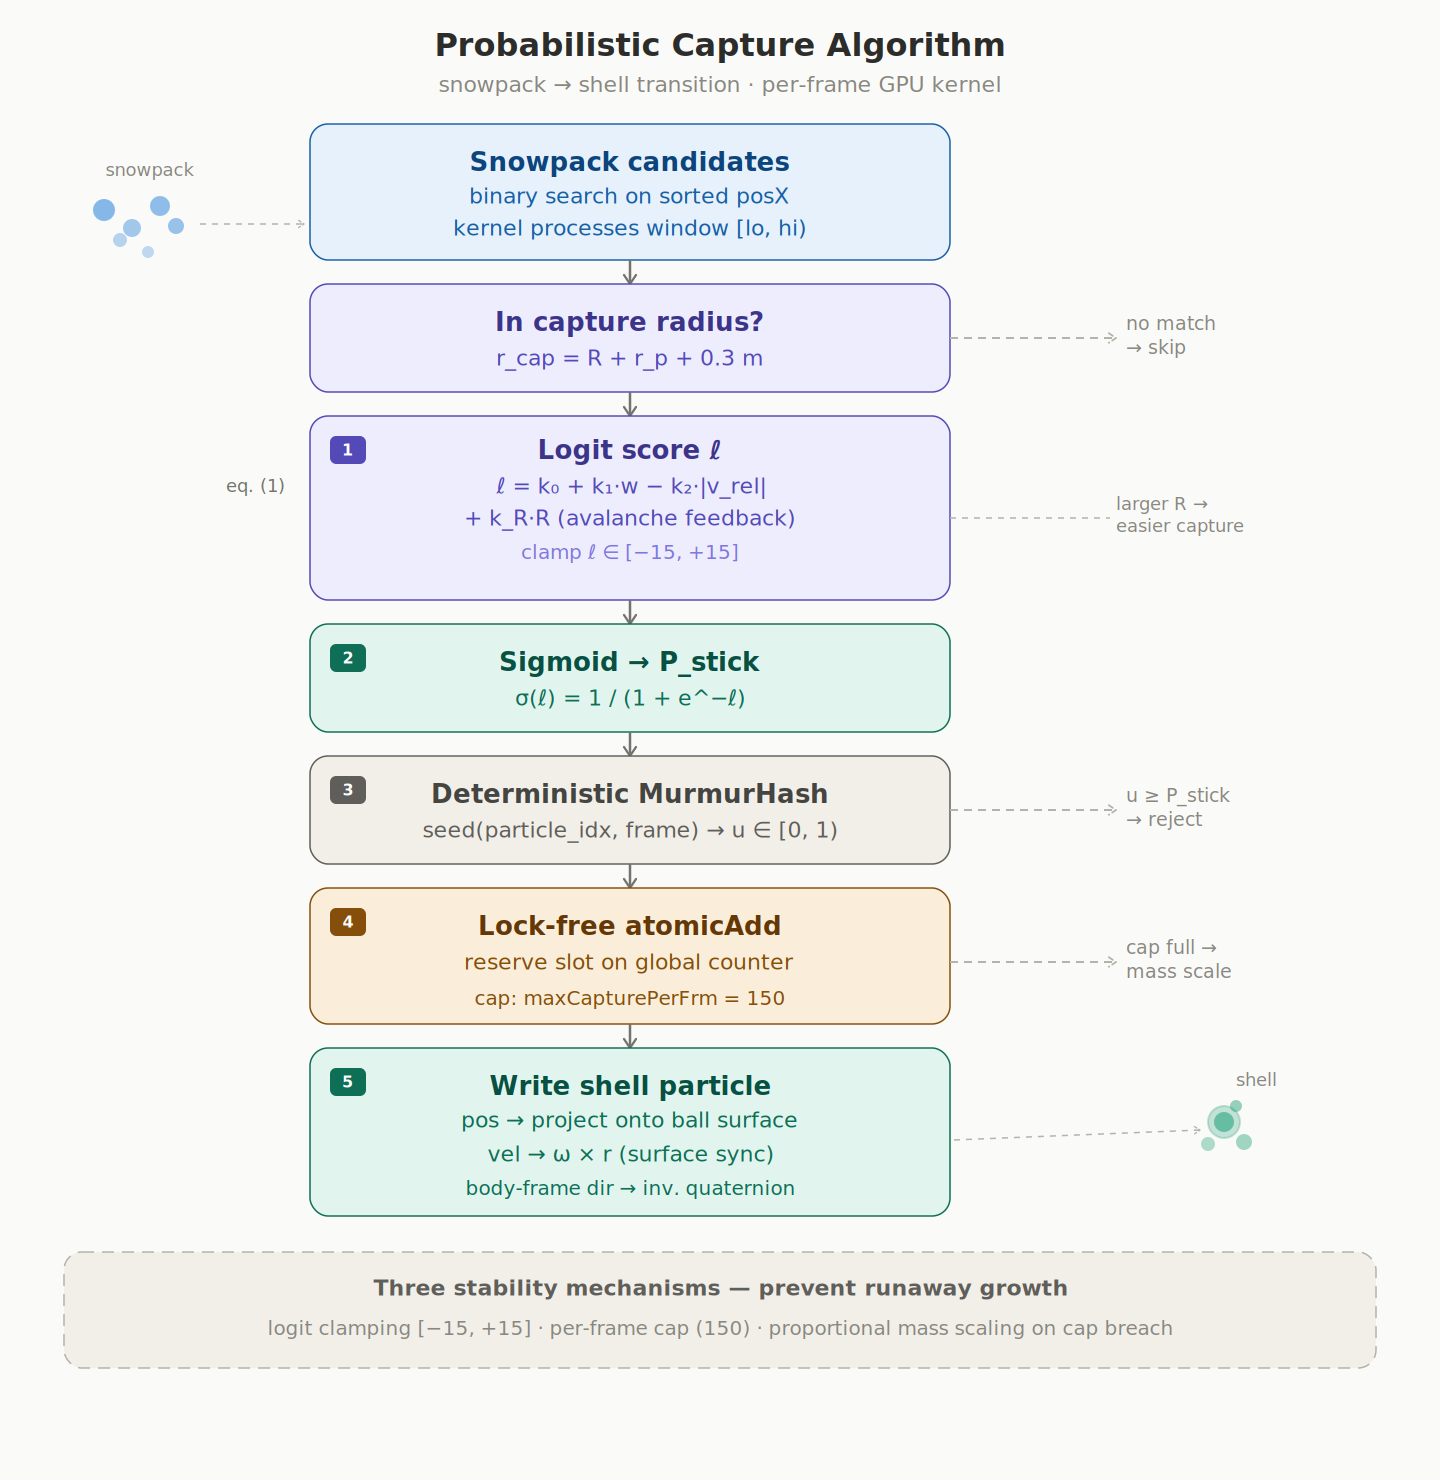
\includegraphics[width=0.9\columnwidth]{figures/capture_diagram.png}}
  \caption{The probabilistic capture algorithm overview. A binary search
  narrows the launch domain; each thread evaluates a sigmoid probability and
  reserves a shell slot via \texttt{atomicAdd} increasing the capacity.}
  \label{fig:capture}
\end{figure}

\subsection{Shell Particle Forces}
\label{sec:forces}

Each shell particle accumulates four force contributions:

\begin{enumerate}
  \item \textbf{Gravity}: $\mathbf{F}_g = m\,(0, -g, 0)$.
  \item \textbf{Mass-proportional damping}: $\mathbf{F}_d = -k_d \cdot m
        \cdot \mathbf{v}$.
  \item \textbf{Tether spring-damper} to the ball surface anchor:
        %
        \begin{equation}
          \mathbf{F}_{\text{tether}} = K(\mathbf{x}_{\text{tgt}} - \mathbf{x})
          + D(\mathbf{v}_{\text{tgt}} - \mathbf{v}),
          \label{eq:tether}
        \end{equation}
        %
        where the target position is computed from the ball's quaternion
        and each particle's body-frame attachment direction.
  \item \textbf{DEM contact} (computed in a separate collision kernel):
        soft-sphere penalty with Coulomb tangential friction
        ($|\mathbf{F}_t| \leq \mu_p |\mathbf{F}_n|$) and short-range
        cohesion for overlapping pairs.
\end{enumerate}

\subsection{Integration and Ground Collision}
\label{sec:integration}

A \textbf{semi-implicit (symplectic) Euler} scheme updates velocity then
position:
%
\begin{equation}
  \mathbf{v}^{n+1} = \mathbf{v}^n + \frac{\mathbf{F}}{m}\Delta t, \qquad
  \mathbf{x}^{n+1} = \mathbf{x}^n + \mathbf{v}^{n+1}\Delta t.
  \label{eq:euler}
\end{equation}
%
Ground collision resolves penetration against the inclined plane with normal
restitution ($e = 0.15$) and Coulomb friction ($\mu = 0.14$). When particles
are captured, the ball velocity is scaled to conserve linear momentum:
$\mathbf{v}' = \frac{m_{\text{old}}}{m_{\text{old}} + \Delta m}\,\mathbf{v}$.
